\documentclass[]{article}

\usepackage{graphicx}

\usepackage[margin=1in]{geometry}

\setlength\parindent{0pt}

\usepackage{physics}
\usepackage{amsmath}
\usepackage{amsfonts}
\usepackage{amssymb}

\usepackage{listings}

\usepackage{enumitem}
\renewcommand{\theenumi}{\alph{enumi}}
\renewcommand*{\thesection}{Problem \arabic{section}}
\renewcommand*{\thesubsection}{\arabic{section}\alph{subsection})}
\renewcommand*{\thesubsubsection}{\quad \roman{subsubsection})}

%Custom Commands
\newcommand{\Rel}{\mathcal{R}}
\newcommand{\R}{\mathbb{R}}
\newcommand{\C}{\mathbb{C}}
\newcommand{\N}{\mathbb{N}}
\newcommand{\Z}{\mathbb{Z}}
\newcommand{\Q}{\mathbb{Q}}

\newcommand{\toI}{\xrightarrow{\textsf{\tiny I}}}
\newcommand{\toS}{\xrightarrow{\textsf{\tiny S}}}
\newcommand{\toB}{\xrightarrow{\textsf{\tiny B}}}


%opening

\title{MATH 5301 Elementary Analysis - Homework 3}

\author{Jonas Wagner}

\date{2021, September 17}



\begin{document}

\maketitle

% Problem 1
\section{}
Let $X$ denote the universal set. Two subsets $A$ and $B$ are said to have 
the same cardinality if there is a bijection $f : A \to B$.
Notation: $\abs*{A} = \abs*{B}$.

\subsection{
	Prove that $\abs{A} = \abs{B}$ is an equivalence relation on the power set of $X$
}

The relation $\Rel = ``\abs{A} = \abs{B}''$
\footnote{using $\Rel$ for simplicyity/reusability} 
is defined as: 
$$\Rel = ``\abs{A} = \abs{B}'' = \{(A,B) : \exists (f : A \xrightarrow{\textsf{\tiny B}} B)\}$$

Equivilence can be demonstrated by proven by demonstrating: 
(i) Reflexivity, (ii) Symetry, and (iii) Transivity


\subsubsection{Reflective:}
\begin{align*}
	A \Rel A
		&= \{(A,A) : \exists (f : A \toB A)\}
\end{align*}
Since $f : A \toB A = {a \in A}$ is true $\forall A \in 2^X$, $\R$ is Reflective.

\subsubsection{Symetric:}
\begin{align*}
	A \Rel B 
		&\implies B \Rel A\\
	\{(A,B) : \exists (f : A \xrightarrow{\textsf{\tiny B}} B)\}
		&\implies \{(B,A) : \exists (f : B \xrightarrow{\textsf{\tiny B}} A)\}
\end{align*}
Since $f : A \toB B \implies g : B \toB A = f^{-1}$ is true $\forall A,B \in 2^X$, 
$\R$ is Symetric.\\
(Essentially if $f$ is bijective one way, 
$f^{-1}$ is bijective for the other way)

\subsubsection{Transative:}
\begin{align*}
	(A \Rel B) 
		\land (B \Rel C) 
		&\implies A \Rel C\\
	(\{(A,B) : \exists (f : A \xrightarrow{\textsf{\tiny B}} B)\})
		\land \{(B,C) : \exists (g : B \xrightarrow{\textsf{\tiny B}} C)\}
		&\implies \{(A,C) : \exists (h : A \xrightarrow{\textsf{\tiny B}} C)\}
\end{align*}
Since $(f : A \toB B) \land (g : B \toB C) 
\implies (h : A \toB C = A \xrightarrow{f} B \xrightarrow{g} C)$ 
is true $\forall A,B,C \in 2^X$, $\Rel$ is Transative.\\

Therefore $\Rel = ``\abs{A} = \abs{B}''$ is an equivalence relation over $2^X$.

\newpage
\subsection{
	Is it true that if $\abs{A_1}=\abs{B_1}$ and $\abs{A_2}=\abs{B_2}$ 
	then $\abs{A_1 \cup A_2} = \abs{B_1 \cup B_2}$?
}
\begin{align*}
	(\abs{A_1} = \abs{B_1}) \land (\abs{A_2} = \abs{B_2})
		&\implies \abs{A_1 \cup A_2} = \abs{B_1 \cup B_2}\\
	(A_1 \Rel B_1) \land (A_2 \Rel B_2)
		&\implies (A_1 \cup A_2) \Rel (B_1 \cup B_2)\\
	\{(A_1,B_1) : \exists (f_1 : A_1 \xrightarrow{\textsf{\tiny B}} B_1)\}
		\land \{(A_2,B_2) : \exists (f_2 : A_2 \xrightarrow{\textsf{\tiny B}} B_2)\}
		&\implies \{((A_1 \cup A_2), (B_1 \cup B_2)) 
			: \exists (f : (A_1 \cup A_2) \xrightarrow{\textsf{\tiny B}} (B_1 \cup B_2))\}
\end{align*}

This itself is false, as in the case when 
\begin{align*}
	(A_1 \cap A_2 \neq \emptyset) \land (B_1 \cap B_2 = \emptyset)
	\implies (f : (A_1 \cup A_2) \toI (B_1 \cup B_2))
	\land (f^{-1} : (B_1 \cup B_2) \toS (B_1 \cup B_2))
\end{align*}
But, $f$ is not surjective and $f^{-1}$ is not injective, so $f$ cannot be bijective.

\newpage
% Problem 2
\section{}
Finish the proof of the Cantor-Bernstein theorem:
For the sets $A$ and $B$, such that $\abs{A} \leq \abs{B}$ and $\abs{B} \leq \abs{A}$
define $A_\infty$ as the set of all elements of $A$ having infinite order,
$A_0$ as the set of all elements of $A$ having even order,
and $A_1$ the set of all elements of $A$ having odd order. Similarly for $B$.

Let
$$A,B : (\abs*{A} \leq \abs*{B}) \land (\abs*{B} \leq \abs*{B})$$

Define
\begin{align*}
	A_\infty &= \{a \in A : \order*{a} = \infty\}\\
	A_0 &= \{a \in A : \order*{a} = 0\}\\
	A_1 &= \{a \in A : \order*{a} = 1\}\\
	B_\infty &= \{b \in B : \order*{b} = \infty\}\\
	B_0 &= \{b \in B : \order*{b} = 0\}\\
	B_1 &= \{b \in B : \order*{b} = 1\}\\
\end{align*}

\subsection{Show that $\abs{A_\infty}=\abs{B_\infty}$.}






\subsection{Construct an injective mapping $A_1 \rightarrow B_0$.}






\subsection{Show that this mapping is also surjective.}





\newpage
% Problem 3
\section{}
Set $A$ is called countable if $\abs{A}\leq \abs{\N}$.
Prove that the following sets are countable.

\subsection{Set $\Z_+$ of all non-negative integer numbers}



\subsection{Set $2\N$ of all even numbers}



\subsection{Set $\Z^2$ of all ordered pairs of integer numbers}



\subsection{Set $\Q$ of all rational numbers}



\subsection{Set $\Q^2$ of all ordered pairs of rational numbers}






\newpage
% Problem 4
\section{}
Prove that the following sets are countable.

\subsection{Set $\mathbf{P}_5(\Z)$ of all polynomials of degree 4 with integer coefficients}


\subsection{Any collection of non-intersecting discs on a plane}



\subsection{Any collection of non-intersecting T-shapes on a plane}
\textbf{Note:} T-shape consists of two perpendicular line segments such that 
one of the segments is attached by one of its endpoints to the center of the other segment. 
The lengths of these segments can be arbitrary. The orientation of the T-shape can be arbitrary.




\subsection{Set $\mathbb{P}$ of all prime numbers}



\subsection{Set $\mathbb{A}$ of all algebraic numbers}
\textbf{Note:} Algebraic numbers are numbers which are roots of 
some polynomials with integer coefficients.








\newpage
% Problem 5
\section{}
Prove that for any infinite set $A$ there exists $B \subset A$, so that $\abs{B}=\abs{\N}$.










\newpage
% Problem 6
\section{}
Prove that the following sets have the same cardinality.
\begin{figure}[h]
	\centering
	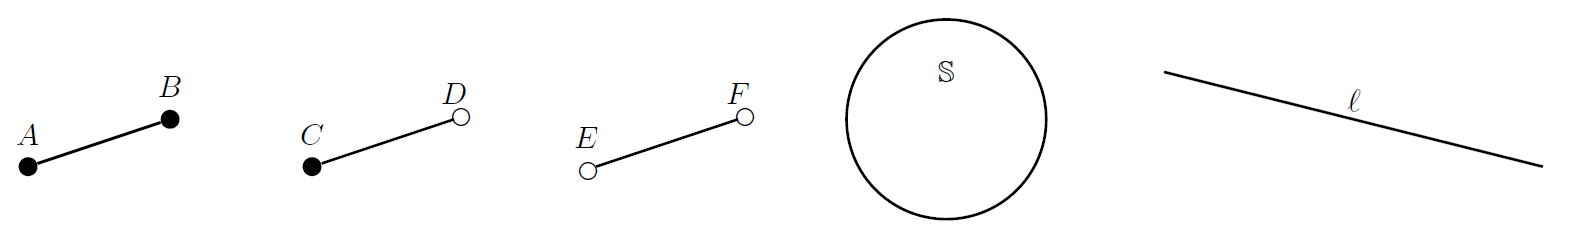
\includegraphics[width=\textwidth]{fig/pblm6.png}
\end{figure}

These sets can all be represented as a set of real number ordered pairs.\\
These are constructed with arbritrary constants: 
$x_a,x_b,x_c,x_d,x_e,x_f,y_a,y_b,y_c,y_d,y_e,y_f,x_s,y_s,r_s,m_l,b_l$

\begin{align*}
	AB &= \{(x,y) \in \R^2, \ t \in \R : 
	(x = (1-t) x_a + t x_b) \land (y = (1-t) y_a + t y_b)
	\land (0 \leq t \leq 1)\}\\
	CD &= \{(x,y) \in \R^2, \ t \in \R : 
	(x = (1-t) x_c + t x_d) \land (y = (1-t) y_c + t y_d)
	\land (0 \leq t < 1)\}\\
	EF &= \{(x,y) \in \R^2, \ t \in \R : 
	(x = (1-t) x_e + t x_f) \land (y = (1-t) y_e + t y_f)
	\land (0 < t < 1)\}\\
	\mathbb{S} &= \{(x,y) \in \R^2, \ t \in \R : 
	(x = r_s cos(2 \pi t) + x_s) \land (y = sin(2 \pi t) + y_s)
	\land (0 \leq t < 1)\}\\
	\mathit{l} &= \{(x,y) \in \R^2, \ t \in \R: (x = t) \land (y = m_l t + b_l)\}
\end{align*}

It is clear that each set is defined parmetrically with bijective equations maping 
the parameter $t$ into a 2-D corndates $(x,y)$, thus proving that the cardinality 
of each sets parameter is sufficent to showing the each set has the same cardinality.\\

Let $T_i = \{t \in A_i\}$ for each of the sets $A_i$, then (from the reasoning above) 
the following can be said:

\begin{align*}
	T_{AB} &= \{t \in \R : 0 \leq t \leq 1\}, \ &\abs{T_{AB}} = \abs{AB}\\
	T_{CD} &= \{t \in \R : 0 \leq t < 1\}, \ &\abs{T_{CD}} = \abs{CD}\\
	T_{EF} &= \{t \in \R : 0 < t < 1\}, \ &\abs{T_{EF}} = \abs{EF}\\
	T_{\mathbb{S}} &= \{t \in \R : 0 \leq t < 1\}, \ &\abs{T_{\mathbb{S}}} = \abs{\mathbb{S}}\\
	T_{\mathit{l}} &= \{t \in \R\}, \ &\abs{T_{\mathit{l}}} = \abs{\mathit{l}}\\
\end{align*}

Clearly, the equivalent definition of $T_{CD}$ and $T_{\mathbb{S}}$ indicates
$$\abs*{CD} = \abs*{T_CD} = \abs*{T_\mathbb{S}} = \abs*{\mathbb{S}}$$

The equivalence of the other sets is more difficult then via definition.\\
First, the baseline cardinality can be shown to be $\aleph_1$ as (by definition of $T_{\mathit{l}})$)
$$\abs{T_\mathit{l}} = \abs{\R} = \aleph_1$$

Next, the equivalence of $T_{EF}$ and $T_\mathit{l}$ can be shown with the biforjective mapping 
$$f_1 : \R \rightarrow T_{EF} = \frac{2 \pi \tan^{-1}(x) + 1}{2}$$
Therefore,
$$\abs{EF} = \abs{T_{EF}} = \abs{T_{\mathit{l}}} = \abs{\R} = \aleph_1$$

Next, due to the nature of infinite sets, the addition of $t=0$ from $T_{EF}$ to $T_{CD}$ 
does not affect the overall cardinality of $T_{CD}$, thus
$$\abs{CD} = \abs{T_{CD}} = \abs{T_{EF}} = \abs{\R} = \aleph_1$$

Similarly, the addition of $t=1$ from $T_{CD}$ to $T_{AB}$ will stil result in 
$$\abs{AB} = \abs{T_{AB}} = \abs{T_{CD}} = \abs{\R} = \aleph_1$$

Ultimently this means that
$$\abs{AB} = \abs{CD} = \abs{EF} = \abs{\mathbb{S}} = \abs{\mathit{l}} = \abs{\R} = \aleph_1$$



\end{document}
